\documentclass[xcolor=table]{beamer}
\usepackage{beamerthemesplit}
\usepackage{wrapfig}
\usetheme{SPbGU}
\usepackage{pdfpages}
\usepackage{amsmath}
\usepackage{amssymb}
\usepackage{cmap}
\usepackage[T2A]{fontenc}
\usepackage[utf8]{inputenc}
\usepackage[english]{babel}
\usepackage{indentfirst}
\usepackage{tikz}
\usetikzlibrary{shapes,arrows,automata,positioning,quotes,backgrounds,decorations.text,decorations.pathmorphing}
\usepackage{multirow}
\usepackage[noend]{algpseudocode}
\usepackage{algorithm}
\usepackage{algorithmicx}
\usepackage{fancyvrb}
\usepackage[linguistics]{forest}
\usepackage{listings}
\usepackage{multicol}
\usepackage{comment}
\usepackage{xspace}
\usepackage{adjustbox}
\usepackage{makecell}
\usepackage{ stmaryrd }

\setbeamertemplate{itemize items}[circle]
\setbeamertemplate{enumerate items}[circle]

\lstdefinelanguage{ocanren}{
keywords={run, conde, fresh, let, match, with, when, class, type,
object, method, of, rec, repeat, until, while, \begin{comment}not,\end{comment} do, done, as, val, inherit,
new, module, sig, deriving, datatype, struct, if, then, else, open, private, virtual, include, success, failure,
true, false},
sensitive=true,
commentstyle=\small\itshape\ttfamily,
keywordstyle=\textbf,%\ttfamily\underline,
identifierstyle=\ttfamily,
basewidth={0.5em,0.5em},
columns=fixed,
mathescape=true,
fontadjust=true,
literate={fun}{{$\lambda$}}1 {function}{function}8 {->}{{$\to$}}3 {<-}{{$\leftarrow$}}3 {===}{{$\equiv$}}1 {=/=}{{$\not\equiv$}}1 {|>}{{$\triangleright$}}3 {\\/}{{$\vee$}}2 {/\\}{{$\wedge$}}2 {^}{{$\uparrow$}}1,
morecomment=[s]{(*}{*)},
 moredelim=**[is][\color{red}]{@!}{@}
}

\tikzstyle{processTree} = [
  ->,
  sibling distance=15em,
  scale=0.6,
  every node/.style = {
    shape=rectangle,
    rounded corners=0.05cm,
    draw,
    align=center,
    minimum size=5mm,
    scale=0.6,},
  %level 1/.style={sibling distance=100em}
  ]


\tikzstyle{program} = [
  draw=black,
  thick,
  rectangle,
  rounded corners=1pt,
  inner sep=5pt,
  inner ysep=5pt
  ]

\tikzstyle{goal} = [
  draw=black,
  rectangle,
  rounded corners=1pt,
  inner ysep=0pt,
  ]

\tikzstyle{input} = [
  draw=none,
  rectangle,
  rounded corners=1pt,
  inner sep=2pt,
  inner ysep=2pt,
  fill=green!10,
  minimum height=5mm
  ]


\tikzstyle{transparent} = [
  draw=none,
  inner ysep=3pt
  ]

\lstset{
language=ocanren
}


\DeclareMathOperator{\Term}{\mathcal{T}}
\DeclareMathOperator{\FlatTerm}{\mathcal{FT}}
\DeclareMathOperator{\Var}{\mathbf{Var}}
\DeclareMathOperator{\Cons}{\mathcal{C}}
\DeclareMathOperator{\Kan}{\mathcal{G}}
\DeclareMathOperator{\Fresh}{\mathbf{Fresh}}
\DeclareMathOperator{\Delay}{\mathbf{Delay}}
\DeclareMathOperator{\Cll}{\mathbf{Call}}
\DeclareMathOperator{\Def}{\mathcal{D}}
\DeclareMathOperator{\Base}{\mathbf{Base}}
\DeclareMathOperator{\Conj}{\mathbf{Conj}}
\DeclareMathOperator{\free}{\mathbf{free}}
\DeclareMathOperator{\ground}{\mathbf{ground}}
\DeclareMathOperator{\In}{\mathbf{In}}
\DeclareMathOperator{\Out}{\mathbf{Out}}
\DeclareMathOperator{\Fun}{\mathcal{F}}
\DeclareMathOperator{\Rtrn}{\mathbf{Return}}
\DeclareMathOperator{\Bind}{\mathbf{Bind}}
\DeclareMathOperator{\Match}{\mathbf{Match}}
\DeclareMathOperator{\Sum}{\mathbf{Sum}}
\DeclareMathOperator{\Guard}{\mathbf{Guard}}
\DeclareMathOperator{\Gen}{\mathbf{Gen}}
\DeclareMathOperator{\Stream}{\mathit{Stream}}
\DeclareMathOperator{\vars}{vars}
\DeclareMathOperator{\inmode}{in}
\DeclareMathOperator{\outmode}{out}
% \DeclareMathOperator{\inmode}{g \rightarrow g}
% \DeclareMathOperator{\outmode}{f \rightarrow g}
% \DeclareMathOperator{\mode1}{mode}
% \DeclareMathOperator{\Mode1}{\mathcal{M}}
\newcommand{\KanN}{\mathcal{K}^{N}}
\newcommand{\tran}[1]{\left\llbracket #1 \right\rrbracket}
\newcommand{\LIST}[1]{\left[ #1 \right]}
\renewcommand{\emptyset}{\varnothing}
\newcommand{\mk}{\textsc{miniKanren}\xspace}
\renewcommand{\and}{$\&$\xspace}
\newcommand{\rel}[2]{\texttt{#1}$^o$ #2}
\newcommand{\subst}[1]{$\langle$#1$\rangle$}
\newcommand{\sem}[1]{\llbracket #1 \rrbracket}

\beamertemplatenavigationsymbolsempty

\title[Functional Conversion for microKanren]{Semi-Automatic Functional Conversion for microKanren}
\institute[JetBrains Research]{
JetBrains Research, Programming Languages and Tools Lab
}

\author[Kate Verbitskaia]{Igor Engel, \textbf{Kate Verbitskaia}}

\date{30.05.2023}

\definecolor{orange}{RGB}{179,36,31}

\begin{document}
{
\begin{frame}[fragile]
   \begin{center}
      
\includegraphics[height=1.5cm]{pictures/jetbrainsResearch.pdf}
    \end{center}
  \titlepage
\end{frame}
}


\begin{frame}[fragile]
  \frametitle{Relational Programming}
\begin{center}
One relation to solve many problems
\end{center}

\begin{center}
Nondeterminism
\end{center}

\begin{center}
Completeness of search
\end{center}

\end{frame}

\begin{frame}[fragile]
  \frametitle{Relational Conversion: Easy}
Given a function
\begin{figure}[!t]
  \centering
  \begin{minipage}{\columnwidth}
    \begin{lstlisting}[label={add_fun},
                      %  caption={Addition function},
                       captionpos=b,
                       frame=tb]
let rec add x y =
  match x with
  | O -> y
  | S x' -> S (add x' y)
    \end{lstlisting}
  \end{minipage}
\end{figure}

generate miniKanren relation
\begin{figure}[!t]
  \centering
  \begin{minipage}{0.7\columnwidth}
    \begin{lstlisting}[frame=tb]
 let rec add$^o$ x y z = conde [
   (x === O /\ y === z);
   (fresh (x$_1$ z$_1$)
     (x === S x$_1$ /\
      add$^o$ x$_1$ y z$_1$ /\
      z === S z$_1$) ) ]
    \end{lstlisting}
  \end{minipage}
\end{figure}
\end{frame}


\begin{frame}[fragile]
  \frametitle{Principal Directions of \mk Relations}
\begin{center}
  Every argument of a relation can be either \lstinline{in} or \lstinline{out}
\end{center}

\begin{center}
  For addition relation \lstinline{add$^o$ x y z} there are 8 directions:
\end{center}

\begin{itemize}
  \item \emph{Forward} direction: \lstinline{add$^o$ in in out} --- addition
  \item \emph{Backward} direction: \lstinline{add$^o$ out out in} --- decomposition
  \item \emph{Predicate}: \lstinline{add$^o$ in in in}
  \item \emph{Generator}: \lstinline{add$^o$ out out out}
  \item \lstinline{add$^o$ in out in} --- subtraction
  \item \lstinline{add$^o$ out in in} --- subtraction
  \item \lstinline{add$^o$ out in out}
  \item \lstinline{add$^o$ in out out}
\end{itemize}
\end{frame}


\begin{frame}[fragile]
  \frametitle{Each Direction is a Function \pause (kinda)}
Straightforward functions:
\begin{itemize}
  \item \emph{Forward} direction: \lstinline{add$^o$ in in out} --- addition
  \item \lstinline{add$^o$ in out in} --- subtraction
  \item \lstinline{add$^o$ out in in} --- subtraction
  \item \emph{Predicate}: \lstinline{add$^o$ in in in}
\end{itemize}

\vfill

Relations:
\begin{itemize}
  \item \emph{Backward} direction: \lstinline{add$^o$ out out in} --- decomposition
  \item \emph{Generator}: \lstinline{add$^o$ out out out}
  \item \lstinline{add$^o$ out in out}
  \item \lstinline{add$^o$ in out out}
\end{itemize}
These relations are functions which return multiple answers (list monad)
\end{frame}

\begin{frame}[fragile]
  \frametitle{\mk Comes with an Overhead}
  \begin{center}
    Unifications
  \end{center}

  \begin{center}
    Occurs-check
  \end{center}

  \begin{center}
    Scheduling complexity
  \end{center}
\end{frame}

\begin{frame}[fragile]
  \frametitle{Functional Conversion}
\begin{center}
  Given a relation and a principal direction, construct a functional program which generates the same answers as \mk would
\end{center}

\vfill

\begin{center}
  Preserve completeness of the search
\end{center}

\vfill

\begin{center}
Both inputs and outputs are expected to be ground
\end{center}
\end{frame}

\lstset{basicstyle=\small}

\begin{frame}[fragile]
  \frametitle{Example: Addition in Forward Direction}
\begin{figure}[!t]
  \centering
  \begin{minipage}{0.7\columnwidth}
    \begin{lstlisting}[frame=tb]
 let rec add$^o$ x y z = conde [
   (x === O /\ y === z);
   (fresh (x$_1$ z$_1$)
     (x === S x$_1$ /\
      add$^o$ x$_1$ y z$_1$ /\
      z === S z$_1$) ) ]
    \end{lstlisting}
  \end{minipage}
\end{figure}

\begin{figure}[!t]
  \centering
  \begin{minipage}{\columnwidth}
    \begin{lstlisting}[frame=tb]
addIIO :: Nat -> Nat -> Nat
addIIO x y =
  case x of
    O -> y
    S x$_1$ -> S (addIIO x$_1$ y)
    \end{lstlisting}
  \end{minipage}
\end{figure}

\end{frame}

\begin{frame}[fragile]
  \frametitle{Addition in Backwards Direction: Nondeterminism}
\begin{figure}[!t]
  \centering
  \begin{minipage}{0.7\columnwidth}
    \begin{lstlisting}[frame=tb]
 let rec add$^o$ x y z = conde [
   (x === O /\ y === z);
   (fresh (x$_1$ z$_1$)
     (x === S x$_1$ /\
      add$^o$ x$_1$ y z$_1$ /\
      z === S z$_1$) ) ]
    \end{lstlisting}
  \end{minipage}
\end{figure}

\begin{figure}[!t]
  \centering
  \begin{minipage}{0.9\columnwidth}
    \begin{lstlisting}[frame=tb,language=ocanren1]
addOOI $::$ Nat -> Stream (Nat, Nat)
addOOI z =
  return (O, z) <$\mid$>
  case z of
    O -> Empty
    S z$_1$ -> do
      (x$_1$, y) <- addOOI z$_1$
      return (S x$_1$, y)
    \end{lstlisting}
  \end{minipage}
\end{figure}

\end{frame}

\begin{frame}[fragile]
  \frametitle{Free Variables in Answers: Generators}
\begin{figure}[!t]
  \centering
  \begin{minipage}{\columnwidth}
    \begin{lstlisting}[label={add},
                      %  caption={Addition relation},
                       captionpos=b,
                       frame=tb]
let rec add$^o$ x y z = conde [
  (x === O /\ y === z);
  (fresh (x' z')
    (x === S x' /\ z === S z' /\ add$^o$ x' y z') ) ]
    \end{lstlisting}
  \end{minipage}
\end{figure}
% \end{frame}

% \begin{frame}[fragile]
%   \frametitle{Free Variables in Answers: Generators}
\begin{figure}[!t]
  \centering
  \begin{minipage}{\columnwidth}
    \begin{lstlisting}[label={add_x},
                      %  caption={Function for \lstinline{addo in out out} direction},
                       captionpos=b,
                       frame=tb]
addX :: Nat -> Stream (Nat, Nat)
addX x = case x of
           O -> do
             z <- genNat
             return (z, z)
           S x' -> do
             (y, z') <- addX x'
             return (y, S z')

genNat :: Stream Nat
genNat = Mature O (S <$\$$> genNat)
    \end{lstlisting}
  \end{minipage}
\end{figure}
\end{frame}

\begin{frame}[fragile]
  \frametitle{Predicates}
  \begin{figure}[!t]
  \centering
  \begin{minipage}{0.7\columnwidth}
    \begin{lstlisting}[frame=tb]
 let rec add$^o$ x y z = conde [
   (x === O /\ y === z);
   (fresh (x$_1$ z$_1$)
     (x === S x$_1$ /\
      add$^o$ x$_1$ y z$_1$ /\
      z === S z$_1$) ) ]
    \end{lstlisting}
  \end{minipage}
\end{figure}

  \begin{figure}[!t]
  \centering
  \begin{minipage}{\columnwidth}
    \begin{lstlisting}[frame=tb]
 addIII $::$ Nat -> Nat -> Nat -> Stream ()
 addIII x y z =
   case x of
     O | y == z -> return ()
       | otherwise -> Empty
     S x$_1$ ->
       case z of
         O -> Empty
         S z$_1$ -> addIII x$_1$ y z$_1$
    \end{lstlisting}
  \end{minipage}
\end{figure}
\end{frame}



\begin{frame}[fragile]
  \frametitle{Conversion Scheme}
  \begin{itemize}
    \item Normalization
    \item Mode analysis
    \item Functional conversion
  \end{itemize}
\end{frame}


\begin{frame}[fragile]
  \frametitle{Normalization: Flat Term}

Flat terms: a var or a constructor which takes distinct vars as arguments:

  \[  \FlatTerm_{V} = V \cup \{\Cons_{i}\left( x_1, \ldots, x_{k_{i}} \right) \mid x_{j}\in V\} \]

Examples:

\[ C\left( x_1, x_2 \right) \equiv C\left( C\left( y_1, y_2 \right), y_3 \right) \iff x_1 \equiv C\left( y_1, y_2 \right) \land x_2 \equiv y_3   \]

\[ C\left( C\left( x_1, x_2 \right), x_3 \right) \equiv C\left( C\left( y_1, y_2 \right), y_3 \right) \iff x_1 \equiv y_1 \land x_2 \equiv y_2 \land x_3 \equiv y_3   \]

\[x \equiv C\left( y, y \right) \iff x \equiv C\left( y_1, y_2 \right)\land y_1 \equiv y_2 \]
\end{frame}



\begin{frame}[fragile]
  \frametitle{Normalization: Goal}
\begin{tabular}{llll}
$\KanN_{V}$ & $=$ & $\bigvee\left( c_1, \ldots, c_{n} \right), c_{i}\in \Conj_{V}$ & normal form \\
$\Conj_{V}$ & $=$ & $\bigwedge\left( g_1, \ldots, g_n \right), g_{i}\in \Base_{V}$ & normal conjunction \\
$\Base_{V}$ & $=$ & $V \equiv \FlatTerm_{V}$ & flat unification \\
            & $\mid$ & $R_{i}^{d}\left( x_1, \ldots, x_{k_{i}} \right), d\in \Delay, x_{j}\in V$ & flat call\\

$\Delay$ & $=$ &  $\{\text{Delay}, \text{NoDelay}\} $ &
\end{tabular}
\end{frame}


\begin{frame}[fragile]
  \frametitle{Mode of a Variable}
Mode of a variable: mapping between its instantiations

\vfill

\emph{Ground} term has no variables

\emph{Free} variable: fresh variable, no info about its instantiation

Once we know that a variable is \emph{ground}, it stays \emph{ground} in subsequent conjuncts

\vfill

Mode $in$: $ground \rightarrow ground$

Mode $out$: $free \rightarrow ground$

\vfill

Mercury uses more complicated modes

\end{frame}

\begin{frame}[fragile]
  \frametitle{Modded Goal}
Assign mode to every variable, make sure they are consistent
\end{frame}

\begin{frame}[fragile]
  \frametitle{Modded Unification}

\begin{itemize}
    \item Assignments: $x^{\outmode}  \equiv \Term^{\inmode}$ and $x^{\inmode} \equiv y^{\outmode}$
    \item Guards: $x^{\inmode} \equiv \Term^{\inmode}$
    \item Match: $x^{\inmode} \equiv \Term$ ($\Term$ contains both \emph{in} and \emph{out} variables)
    \item Generators: $x^{\outmode} \equiv \Term$
\end{itemize}
\end{frame}

\begin{frame}[fragile]
  \frametitle{Mode Inference: Initialization }

\begin{itemize}
  \item For all input variables: $ground \rightarrow ?$
  \item For all other variables: $free \rightarrow ?$
\end{itemize}

\begin{figure}[!t]
  \centering
  \begin{minipage}{\columnwidth}
    \begin{lstlisting}[frame=tb]
let rec add$^o$ x$^{g \to g}$ y$^{g \to g}$ z$^{f \to g}$ = conde
  (x$^{g \to g}$  ===    O /\ y$^{g \to g}$ ===     z$^{f \to g}$);
  (x$^{g \to g}$ ===     S x$_1^{f \to ?}$ /\
   add$^o$ x$_1^{f \to ?}$ y$^{g \to g}$ z$_1^{f \to ?}$ /\
   z$^{f \to g}$ ===     S z$_1^{f \to ?}$)
    \end{lstlisting}
  \end{minipage}
\end{figure}
\end{frame}

\begin{frame}[fragile]
  \frametitle{Mode Inference: Disjunction }
Run inference on each disjunct independently

\begin{figure}[!t]
  \centering
  \begin{minipage}{0.65\columnwidth}
    \begin{lstlisting}[frame=tb]
 x$^{\inmode}$  === O /\ y$^{\inmode}$ ===  z$^{\outmode}$
    \end{lstlisting}
  \end{minipage}
\end{figure}
\begin{figure}[!t]
  \centering
  \begin{minipage}{0.55\columnwidth}
    \begin{lstlisting}[frame=tb]
 x$^{\inmode}$ ===  S x$_1^{\whatmode}$ /\
 add$^o$ x$_1^{\whatmode}$ y$^{\inmode}$ z$_1^{\whatmode}$ /\
 z$^{\outmode}$ ===  S z$_1^{\whatmode}$
    \end{lstlisting}
  \end{minipage}
\end{figure}
\end{frame}


\begin{frame}[fragile]
  \frametitle{Mode Inference: Unification}
Propagate the groundness information according to the 4 types of modded unifications


\begin{figure}[!t]
  \centering
  \begin{minipage}{\columnwidth}
    \begin{lstlisting}[label={add},
                      %  caption={Addition relation},
                       captionpos=b,
                       frame=tb]
  x$^{g \to g}$ ===     S x$_1^{f \to ?}$ $\Rightarrow$ x$^{g \to g}$ ===          S x$_1^{f \to g}$
    \end{lstlisting}
  \end{minipage}
\end{figure}
\begin{figure}[!t]
  \centering
  \begin{minipage}{\columnwidth}
    \begin{lstlisting}[label={add},
                      %  caption={Addition relation},
                       captionpos=b,
                       frame=tb]
  z$^{f \to g}$ ===     S z$_1^{f \to ?}$ $\Rightarrow$ z$^{f \to g}$ ===          S z$_1^{f \to g}$
    \end{lstlisting}
  \end{minipage}
\end{figure}
\end{frame}

\begin{frame}[fragile]
  \frametitle{Mode Inference: Conjunction}
Pick a conjunct according to the priority, propagate groundness
\begin{itemize}
  \item Guards
  \item Assignments
  \item Matches
  \item Calls with at least one ground argument
  \item Generators
\end{itemize}
\end{frame}

\begin{frame}[fragile]
  \frametitle{Mode Inference: Conjunction}
\begin{figure}[!t]
  \centering
  \begin{minipage}{\columnwidth}
    \begin{lstlisting}[label={add},
                      %  caption={Addition relation},
                       captionpos=b,
                       frame=tb]
  x$^{g \to g}$ ===     S x$_1^{f \to ?}$ /\
  add$^o$ x$_1^{f \to ?}$ y$^{g \to g}$ z$_1^{f \to ?}$ /\
  z$^{g \to g}$ ===     S z$_1^{f \to ?}$
    \end{lstlisting}
  \end{minipage}
\end{figure}
\begin{figure}[!t]
  \centering
  \begin{minipage}{\columnwidth}
    \begin{lstlisting}[label={add},
                      %  caption={Addition relation},
                       captionpos=b,
                       frame=tb]
  (((x, g->g) === S (x', f->g) /\
    add$^o$ (x', f->g) (y, g->g) (z', f->?) /\
    (z,f->g) === S (z', f->?)))
    \end{lstlisting}
  \end{minipage}
\end{figure}
\begin{figure}[!t]
  \centering
  \begin{minipage}{0.57\columnwidth}
    \begin{lstlisting}[frame=tb]
 x$^{\inmode}$ ===  S x$_1^{\outmode}$ /\
 add$^o$ x$_1^{\inmode}$ y$^{\inmode}$ z$_1^{\outmode}$ /\
 z$^{\outmode}$ ===  S z$_1^{\inmode}$
    \end{lstlisting}
  \end{minipage}
\end{figure}
\end{frame}

\begin{frame}[fragile]
  \frametitle{Order in Conjunctions}
  \begin{figure}[!t]
  \centering
  \begin{minipage}{\columnwidth}
    \begin{lstlisting}[label={mult},
                      %  caption={Multiplication relation},
                       captionpos=b,
                       frame=tb]
let rec mult$^o$ x y z = conde [
  ...
  (fresh (x' r')
    (x === S x') /\
    (add y r' z) /\
    (mult x' y r')
  )]
    \end{lstlisting}
  \end{minipage}
\end{figure}

\end{frame}

\begin{frame}[fragile]
  \frametitle{Order in Conjunctions: Slow Version}
  \begin{figure}[!t]
  \centering
  \begin{minipage}{\columnwidth}
    \begin{lstlisting}[label={mult_slow}, caption={Inefficient implementation of \lstinline{multo in in out} direciton}, captionpos=b, frame=tb]
multXY' :: Nat -> Nat -> Stream Nat
multXY' O     y     = return O
multXY' x     O     = return O
multXY' (S O) y     = return y
multXY' x     (S O) = return x
multXY' (S x') y    = do
  (r', r) <- addX y
  multXYZ x' y r'
  return r

multXYZ :: Nat -> Nat -> Nat -> Stream ()
multXYZ O      y     O = return ()
multXYZ x      O     O = return ()
multXYZ (S O)  y     z | y == z = return ()
multXYZ x      (S O) z | x == z = return ()
multXYZ (S x') y     z = do
  z' <- multXY' x' y
  addXYZ y z' z
multXYZ _ _ _ = Empty
    \end{lstlisting}
  \end{minipage}
\end{figure}

\end{frame}


\begin{frame}[fragile]
  \frametitle{Order in Conjunctions: Faster Version}
  \begin{figure}[!t]
  \centering
  \begin{minipage}{0.8\columnwidth}
    \begin{lstlisting}[frame=tb]
 multIIO $::$ Nat -> Nat -> Stream Nat
 multIIO (S x$_1$) y = do
   r$_1$ <- multIIO x$_1$ y
   addIIO y r$_1$
 ...
    \end{lstlisting}
  \end{minipage}
\end{figure}

\end{frame}

\begin{frame}[fragile]
  \frametitle{Functional Conversion: Intermediate Language}
\begin{tabular}{llll}
    $\Fun_{V}$ & $=$ &  $\Rtrn \LIST{\Term_{V}}$ & return a tuple of terms\\
               & $\mid$ &  $\Match_{V} \left( \Term_{V}, \Fun_{V} \right)$& match a variable against a pattern\\
               & $\mid$ & $\Bind\LIST{\left(\LIST{V}, \Fun_{V}\right)} $ & monadic bind on streams\\
               & $\mid$ & $\Sum\LIST{\Fun_{V}}$ & concatenation of streams\\
               & $\mid$ & $\Guard\left( V, V \right)$ & equality check\\
               & $\mid$ & $\Gen_{G}$ & generator\\
               & $\mid$ & $R_{i}^{d}(\LIST{V}, \LIST{G}), d\in \Delay $ & function call
\end{tabular}
\end{frame}

\begin{frame}[fragile]
  \frametitle{Functional Conversion into Intermediate Language}
\begin{itemize}
  \item Disjunction $\rightarrow \Sum\LIST{\Fun_{V}}$
  \item Conjunction $\rightarrow \Bind\LIST{\left(\LIST{V}, \Fun_{V}\right)}$
  \item Relation call $\rightarrow R_{i}^{d}(\LIST{V}, \LIST{G}), d\in \Delay$
  \item Unification $\rightarrow \Rtrn \LIST{\Term_{V}}$ or $\Match_{V} \left( \Term_{V}, \Fun_{V} \right)$ or $\Guard\left( V, V \right)$ or $\Gen_{G}$
\end{itemize}
\end{frame}

\begin{frame}[fragile]
  \frametitle{Functional Conversion into Haskell}
  \begin{itemize}
    \item TemplateHaskell to generate code
    \item Stream monad
    \item do-notation
  \end{itemize}
\end{frame}

\begin{frame}[fragile]
  \frametitle{Functional Conversion into OCaml}
  \begin{itemize}
    \item Hand-crafted (not so) pretty-printer
    \item Stream monad
    \item let*
    \item Taking extra care to employ laziness
  \end{itemize}
\end{frame}

\begin{frame}[fragile]
  \frametitle{Evaluation (last year)}
  \begin{center}
    We manually converted relational interpreters and measured execution time
  \end{center}

  \begin{itemize}
    \item Topologic sort
    \begin{itemize}
      \item A verifier verifies that a vertex mapping sorts vertices topologically
      \item Sort a DAG with an edge in between every pair of vertices
      \item Two different representations: vertices sorted by their number, and with a reverse order
      \item Sorting a graph with up to 6 vertices
    \end{itemize}
    \item Logic formulas generation
    \begin{itemize}
      \item Inverse computation of a logic formulas interpreter
      \item Generate 10000 formulas which evaluate to \texttt{true}
      \item Different substitution lengths
    \end{itemize}
  \end{itemize}
\end{frame}

\begin{frame}[fragile]
  \frametitle{Evaluation: Topologic Sort (last year)}
  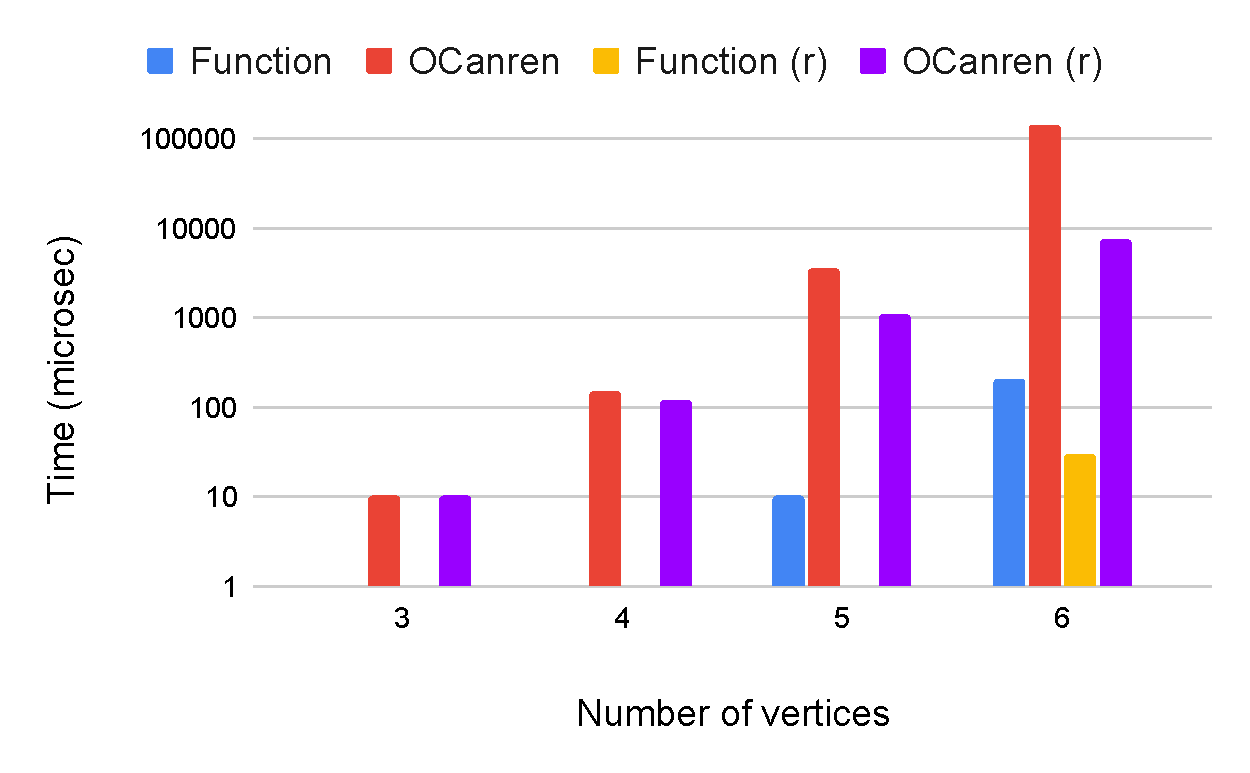
\includegraphics[width=\textwidth]{fig/eval/topsort.pdf}
\end{frame}

\begin{frame}[fragile]
  \frametitle{Evaluation: Logic Formulas Generation (last year)}
  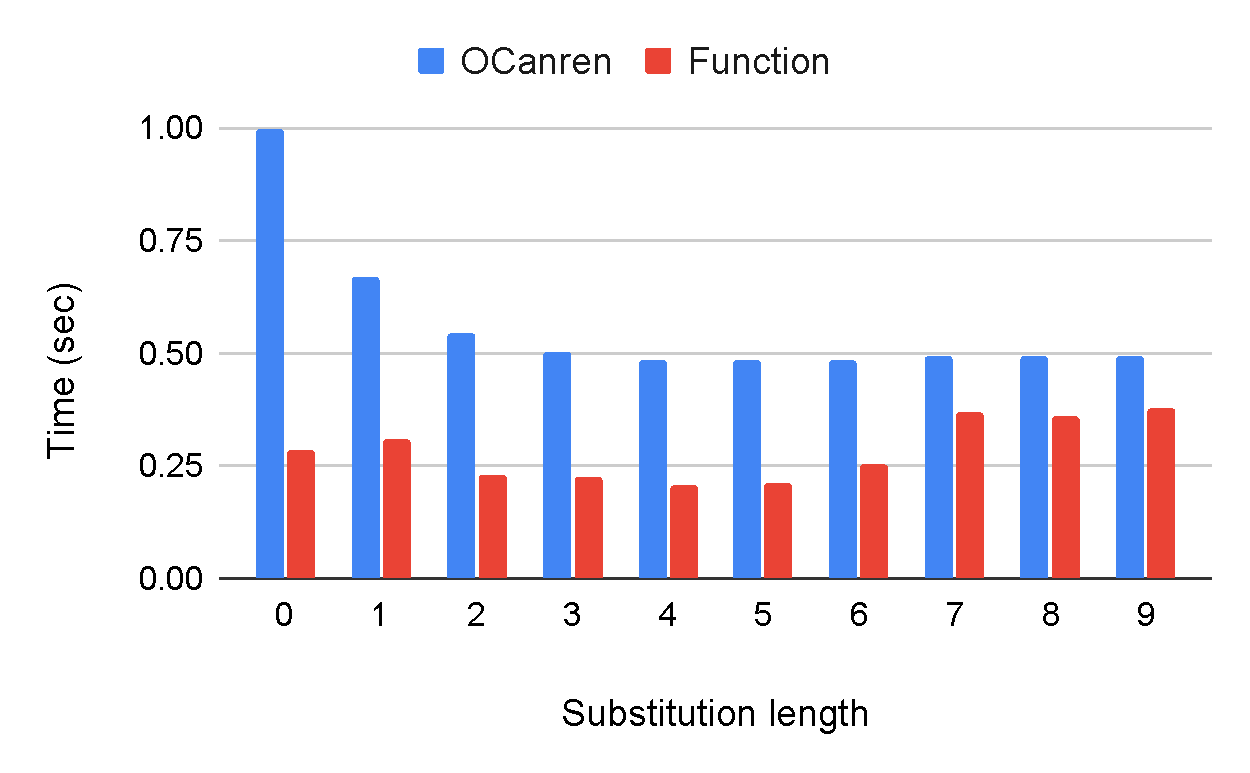
\includegraphics[width=\textwidth]{fig/eval/prop.pdf}
\end{frame}


\begin{frame}[fragile]
  \frametitle{Evaluation: Addition Relation (Time in Seconds)}
\begin{itemize}
  \item addIIO x = 10000, y = 0
  \begin{itemize}
    \item Fun: 0.007
    \item Rel: 1.533
  \end{itemize}
  \item addOII y = 0, z = 10000
  \begin{itemize}
    \item Fun: 0.009
    \item Rel: 1.547
  \end{itemize}
  \item addIOI x = 10000, z = 10000
  \begin{itemize}
    \item 0.009
    \item 3.029
  \end{itemize}
  \item addIII x = 10000, y = 0, z = 10000
  \begin{itemize}
    \item 0.008
    \item 3.041
  \end{itemize}
  \item addIOO x = 0, n = 1000
  \begin{itemize}
    \item Fun: 0.143
    \item Rel: 0.000
  \end{itemize}
  \item addOOO n = 1000
  \begin{itemize}
    \item Fun: 0.074
    \item Rel: 0.585
  \end{itemize}
\end{itemize}
\end{frame}

\begin{frame}[fragile]
  \frametitle{Evaluation: Proposition Evaluator (Time in Seconds)}
\begin{itemize}
  \item evalo [true; false; true] fm true
  \begin{itemize}
    \item Fun: 0.759
    \item Rel: 0.308
  \end{itemize}
\end{itemize}
\end{frame}

\begin{frame}[fragile]
  \frametitle{Data Types}
We generate weird data type declarations:
\begin{figure}[!t]
  \centering
  \begin{minipage}{\columnwidth}
    \begin{lstlisting}[label={add},
                      %  caption={Addition relation},
                       captionpos=b,
                       frame=tb]
type term =
  | Conj of (term* term)
  | Cons of (term* term)
  | Disj of (term* term)
  | Falso
  | Neg of term
  | Succ of term
  | Trueo
  | Var of term
  | Zero
        \end{lstlisting}
  \end{minipage}
\end{figure}

\begin{figure}[!t]
  \centering
  \begin{minipage}{\columnwidth}
    \begin{lstlisting}[label={add},
                      %  caption={Addition relation},
                       captionpos=b,
                       frame=tb]
elem$^o$ i st v =
  fresh (h t i') conde [
    (i === Zero /\ st === Cons (v, t));
    (i === Succ i' /\ st === Cons (h, t) /\ elem$^o$ i' t v)]
      \end{lstlisting}
  \end{minipage}
\end{figure}
\end{frame}

\begin{frame}[fragile]
  \frametitle{Need for Determinism Check}
  \begin{itemize}
    \item Replacing Stream with Maybe improves performance about 10 times for relations on natural numbers
    \item Functional (no monad) version is still faster
    \item Use determinism check to figure out when replacing Stream is feasible
    \item How to combine different monads naturally?
  \end{itemize}
\end{frame}



\begin{frame}[fragile]
  \frametitle{Need for Partial deduction}

\begin{center}
\mk can run a verifier backwards to get solver
\end{center}

\begin{center}
\begin{minipage}{0.3\textwidth}
  \lstinline{run q (eval$^o$ q true)}
\end{minipage}

\begin{center}
  Augmenting functional conversion with partial deduction must be beneficial
\end{center}
\end{center}


\end{frame}


\begin{frame}[fragile]
  \frametitle{Conclusion}
Conclusion
  \begin{itemize}
    \item We presented a functional conversion scheme as a series of examples
    \item The conversion speeds up implementations considerably
    \item We implemented the conversion scheme in Haskell
    \item Found some way to order conjuncts
  \end{itemize}

\vfill

Future work
  \begin{itemize}
    \item Integration with partial deduction
    \item Integration into a relational interpreters for solving framework
  \end{itemize}
\end{frame}




% \begin{frame}[fragile]
%   \frametitle{Solvers from Verifiers}
% \begin{center}
%   An inverse of a verifier is a solver
% \end{center}

% \begin{center}
%   Verifier is much easier to implement than a solver
% \end{center}
% \end{frame}


% \begin{frame}[fragile]
%   \frametitle{Inverse Computations}
% \begin{center}
% Given a program $p$:
% \end{center}
% $$
% \sem{p} x = y
% $$

% \begin{center}
% Its inversion is:
% \end{center}
% $$
% \sem{p^{-1}} y = x
% $$

% \vfill


% \begin{center}
% Program inverter:
% \end{center}
% $$
% \sem{invtrans} p = p^{-1}
% $$

% \begin{center}
% Inverse interpreter:
% \end{center}
% $$
% \sem{invint} [p, y] = x
% $$

% \end{frame}


% \begin{frame}[fragile]
%   \frametitle{\mk Works as an Inverse Interpreter}

% \begin{center}
% \mk can run a verifier backwards
% \end{center}

% \begin{center}
% \begin{minipage}{0.3\textwidth}
%   \lstinline{run q (eval$^o$ q true)}
% \end{minipage}
% \end{center}


% \end{frame}



% \begin{frame}[fragile]
%   \frametitle{Partial Deduction for \mk: Bird's-eye View}
%   \begin{center}
% \lstset{language=ocanren1}
\begin{tikzpicture}[
  node distance = 14mm and 13 mm,
  decoration = {
    snake,
    pre length=2pt,
    post length=4pt,
    amplitude=0.5pt,
    segment length=4pt
  },
  remember picture,overlay]
  \node (a) [
    program,
    anchor=north west,
    xshift=1cm,
    yshift=-1.3cm]
  at (current page.north west)
  {
    \adjustbox{scale=0.65}{
      \begin{minipage}[c]{0.38\textwidth}
        \begin{lstlisting}
let rec eval$^o$ fm s r =
  ...
  fm === conj x y /\
  and$^o$ a b r /\
  eval$^o$ x s a /\
  eval$^o$ y s b \/
  ...
        \end{lstlisting}
      \end{minipage}
    }
  };

  \node (b) [goal,anchor=north east] at (a.south east)
  {
    \adjustbox{scale=0.65}{
      \begin{minipage}[c]{0.24\textwidth}
        \begin{lstlisting}
eval$^o$ fm s true
        \end{lstlisting}
      \end{minipage}
    }
  };

  \pause

  \node (d) [
    transparent,
    xshift=-1cm,
    yshift=-1.3cm,
    anchor=north east]
  at (current page.north east)
  {
      \begin{tikzpicture}[
  processTree,
  sibling distance=7em,
  level distance=7em,
  level 2/.style={level distance=5em},
  anchor=center]
  \node {
    \rel{eval}{$fm \ s \ true$}}
    child { node[draw=none, fill=none] {...}}
    child { node {
      \rel{and}{$a \ b \ true$} $\wedge$  \\
      \rel{eval}{$x \ s \ a$} $\wedge$ \\
      \rel{eval}{$y \ s \ b$} \\
      \subst{$fm \to conj \ x \ y$}} 
      child { node[draw=none, fill=none] {...}}
      }
    child { node[draw=none, fill=none] {...}}
  ;
\end{tikzpicture}
  };

  \draw[->,semithick, decorate]
    ($(a.north east)+(0,-1)$) to
    [out=15,in=165,"{\footnotesize driving}"]
    ($(d.north west)+(0,-1)$);

  \pause

  \node (e) [transparent, anchor=north] at ($(d.north)+(0.3,-4.3)$)
  {
    \begin{minipage}[c]{0.4\textwidth}
      \begin{tikzpicture}[
  processTree,
  sibling distance=4em,
  level distance=3em,
  level 3/.style={level distance=4em,sibling distance=8em},
  anchor=center]
  \node (root) {
    \rel{eval}{$fm \ s \ true$}}
    child { node[draw=none, fill=none] {...}}
    child { node[draw=none, fill=none] {...}
      child { node {
        \rel{eval}{$x \ s \ true$} $\wedge$ \\
        \rel{eval}{$y \ s \ true$}}
        child { node (1) {\rel{eval}{$x \ s \ true$}}}
        child { node (2) {\rel{eval}{$y \ s \ true$}}}
        }
    }
    child { node[draw=none, fill=none] {...}}
  ;

  \draw [dashed,->] (1.west) to [out=170,in=-150] (root.west);
  \draw [dashed,->] (2.east) to [out=10,in=-30] (root.east);


\end{tikzpicture}
    \end{minipage}
  };

  \draw[->,semithick, decorate]
    ($(d.south)+(0.5,0.3)$) to
    [out=-75,in=75,"{\footnotesize folding}"]
    ($(e.north)+(0.2,0)$);

  \pause

  \node (c) [
    program,
    anchor=south west,
    xshift=1cm,
    yshift=0.8cm]
  at (current page.south west)
  {
    \adjustbox{scale=0.65}{
      \begin{minipage}[c]{0.4\textwidth}
        \begin{lstlisting}
let rec eval$^o$_true fm s =
  ...
  fm === conj x y /\
  eval$^o$_true x s /\
  eval$^o$_true y s \/
  ...
        \end{lstlisting}
      \end{minipage}
    }
  };

  \draw[->,semithick, decorate]
    ($(e.west)+(0.45,0)$) to
    [out=200,in=-20,"{\footnotesize residualization}",pos=0.5]
    (c.east);

    \onslide<1->
\end{tikzpicture}
%   \end{center}
% \end{frame}

% \begin{frame}[fragile]
%   \frametitle{Driving: Unfolding}
%   \begin{center}
%     \input{drivingUnfold.tex}
%   \end{center}
% \end{frame}

% \begin{frame}[fragile]
%   \frametitle{Partial Deduction}

% \begin{center}
%   \input{pd2.tex}
% \end{center}

% \end{frame}

% \begin{frame}[fragile]
%   \frametitle{Conjunctive Partial Deduction: Left-to-right Unfolding}

% \begin{center}
%   \input{cpd2.tex}
% \end{center}
% \end{frame}


% \begin{frame}[fragile]
%   \frametitle{CPD: Split is Necessary}
% \begin{center}
%   \input{splitNecessary.tex}
% \end{center}
% \end{frame}

% \begin{frame}[fragile]
%   \frametitle{Split: Which Way is the Right Way?}
% \input{split.tex}
% \end{frame}

% \begin{frame}[fragile]
%   \frametitle{Decisions in Partial Deduction}
% \begin{itemize}
%   \item What to unfold: which calls, how many calls?
%   \begin{itemize}
%     \item CPD: the leftmost call, which does not have a predecessor \emph{embedded} into it
%   \end{itemize}
%   \item How to unfold: to what depth a call should be unfolded?
%   \begin{itemize}
%     \item CPD: unfold once
%   \end{itemize}
%   \item When to stop driving?
%   \begin{itemize}
%     \item When a goal is an instance of some goal in the process tree
%   \end{itemize}
%   \item When to split?
%   \begin{itemize}
%     \item When there is a predecessor embedded into the goal
%   \end{itemize}
% \end{itemize}
% \end{frame}

% \begin{frame}[fragile]
%   \frametitle{Evaluator of Logic Formulas: Unfolding Step 1}

% \begin{tikzpicture}[
%   remember picture,
%   overlay
% ]
%   \node (a) [
%     program,
%     anchor=north west,
%     xshift=0.4cm,
%     yshift=-1.4cm
%   ]
%   at (current page.north west)
%   {
%     \adjustbox{scale=0.6}
%     {
%       \begin{minipage}[c]{\textwidth}
%         \lstset{language=ocanren1}

\begin{lstlisting}
let rec eval$^o$ fm s r =
  fresh (v x y a b) (
    (fm === var v /\ lookup$^o$ v s r) \/
    (fm === neg x /\ eval$^o$ x s a /\ not$^o$ a r) \/
    (fm === conj x y /\ eval$^o$ x s a /\ eval$^o$ y s b /\ and$^o$ a b r) \/
    (fm === disj x y /\ eval$^o$ x s a /\ eval$^o$ y s b /\ or$^o$ a b r) )
  \end{lstlisting}
%       \end{minipage}
%     }};

%   \node [
%       goal,
%       anchor=north east,
%     ]
%     at (a.south east)
%     {
%       \adjustbox{scale=0.6}
%       {
%         \begin{minipage}[c]{0.25\textwidth}
%           \begin{lstlisting}
% eval$^o$ fm s true
%           \end{lstlisting}
%         \end{minipage}
%       }};

%   \node [
%     transparent,
%     anchor=south,
%     yshift=1cm,
%   ]
%   at (current page.south)
%   {
%       \input{propCPD.tex}
%   };
% \end{tikzpicture}

% \end{frame}


% \begin{frame}[fragile]
%   \frametitle{Evaluator of Logic Formulas: Unfolding Step 2}

% \begin{center}
%   \input{propCPDunf2.tex}
% \end{center}
% \end{frame}

% \begin{frame}[fragile]
%   \frametitle{Unfolding of Boolean Connectives}

%   \begin{center}
%     \input{boolOr.tex}
%   \end{center}

%   \vspace{1cm}

%   \begin{columns}
%     \begin{column}{0.5\textwidth}
%       \begin{center}
%         \input{boolNot.tex}
%       \end{center}
%     \end{column}
%     \begin{column}{0.5\textwidth}
%       \begin{center}
%         \input{boolAnd.tex}
%       \end{center}
%     \end{column}
%   \end{columns}
% \end{frame}


% \begin{frame}[fragile]
%   \frametitle{Unfolding Boolean Connectives First}

% \begin{center}
%   \input{propCPDunf3.tex}
% \end{center}
% \end{frame}

% \begin{frame}[fragile]
%   \frametitle{Evaluator of Logic Formulas: Conservative PD}

% \begin{center}
%   \begin{tikzpicture}[
  processTree,
  level 1/.style={sibling distance=21em, level distance=7em},
  level 2/.style={sibling distance=10em},
  level 3/.style={level distance=6em},
  level 4/.style={level distance=4em},
  level 5/.style={sibling distance=2em, level distance=4em},
  level distance=8em]
  \node (root) {
    \underline{\rel{eval}{$fm \ s \ true$}}}
    child { node {
      \rel{eval}{$x \ s \ a$} $\wedge$ \\
      \underline{\rel{not}{$a \ true$}} \\
      \subst{$fm \to neg \ x$}}
      child { node (1) {
        \rel{eval}{$x \ s \ false$} \\
        \subst{$a \to false$}}}}
    child { node {
      \rel{eval}{$x \ s \ a$} $\wedge$ \\
      \rel{eval}{$y \ s \ b$} $\wedge$ \\
      \underline{\rel{or}{a \ b \ true}} \\
      \subst{$fm \to disj \ x \ y$}}
      child { node {
        \rel{eval}{$x \ s \ true$} $\wedge$ \\
        \rel{eval}{$y \ s \ true$} \\
        \subst{$a \to true, b \to true$}}}
      child { node {
        \rel{eval}{$x \ s \ true$} $\wedge$ \\
        \rel{eval}{$y \ s \ false$} \\
        \subst{$a \to true, b \to false$}}
        child { node [diamond] { $\wedge$ }
          child { node (rename) {
            \rel{eval}{$x \ s \ true$}}}
          child { node (2) {
            \rel{eval}{$y \ s \ false$}}
            child { node[draw=none, fill=none] {...}}
            child { node[draw=none, fill=none] {...}}
            child { node[draw=none, fill=none] {...}}
            child { node[draw=none, fill=none] {...}}}}}
      child { node {
        \rel{eval}{$x \ s \ false$} $\wedge$ \\
        \rel{eval}{$y \ s \ true$} \\
        \subst{$a \to false, b \to true$}}}}
    child { node {
      \rel{eval}{$x \ s \ a$} $\wedge$ \\
      \rel{eval}{$y \ s \ b$} $\wedge$ \\
      \underline{\rel{and}{a \ b \ true}} \\
      \subst{$fm \to conj \ x \ y$}}
      child { node {
        \rel{eval}{$x \ s \ true$} $\wedge$ \\
        \rel{eval}{$y \ s \ true$} \\
        \subst{$a \to true, b \to true$}}}}
  ;
  \node[left=8em of root] (lookup) {
    \rel{lookup}{$x \ s \ true$} \\
    \subst{$fm \to var \ v$}
  };
  \draw [->] (root.west) to [out=180,in=0] (lookup.east);
  \pause
  \draw [dashed,<-] ($(root.south west)-(-1,0)$) .. controls +(-7,-2.5) and +(-4,0) .. (rename.west);

  \draw[dashed,->] (1.south) to [out=-90,in=-135] (2.south west);

  \onslide<1->
\end{tikzpicture}
% \end{center}
% \end{frame}

% \begin{frame}[fragile]
%   \frametitle{Conservative Partial Deduction}
% \begin{itemize}
%   \item Split conjunction into individual calls
%   \item Unfold each call in isolation
%   \item Unfold until embedding is encountered
%   \item Find a call which narrows the search space (less-branching heuristics)
%   \item Join the result of unfolding the selected call with the other calls not unfolded
%   \item Continue driving the constucted conjunction
% \end{itemize}

% \end{frame}

% \begin{frame}[fragile]
%   \frametitle{Less-branching Heuristics}

%   \begin{center}
%     Less-branching heuristics is used to select a call to unfold

%     \vspace{0.5cm}

%     If a call in the context unfolds into less branches than it does in isolation, select it
%   \end{center}

% \vspace{0.5cm}


%   \begin{columns}
%     \begin{column}[]{0.65\textwidth}
%       \begin{center}
%         \input{boolAndIso.tex}
%       \end{center}
%     \end{column}
%     \begin{column}[]{0.35\textwidth}
%       \input{boolAnd.tex}
%     \end{column}
%   \end{columns}
% \end{frame}

% \begin{frame}[fragile]
%   \frametitle{Evaluation}
% We implemented the Conservative Partial Deduction and compared it with CPD for \mk and CPD with branching heuristics on the following relations

% \begin{itemize}
%   \item Two implementations of an evaluator of logic formulas
%   \item A program to compute a unifier of two terms
%   \item A program to search for paths of a specific length in a graph
% \end{itemize}
% \end{frame}

% %\begin{frame}[fragile]
% %  \frametitle{Evaluator of Logic Formulas}
% %    \begin{center}
% %      \adjustbox{scale=0.9}
% %      {
% %        \begin{minipage}[c]{\textwidth}
% %          \lstset{language=ocanren1}

\begin{lstlisting}
let rec eval$^o$ fm s r =
  fresh (v x y a b) (
    (fm === var v /\ lookup$^o$ v s r) \/
    (fm === neg x /\ eval$^o$ x s a /\ not$^o$ a r) \/
    (fm === conj x y /\ eval$^o$ x s a /\ eval$^o$ y s b /\ and$^o$ a b r) \/
    (fm === disj x y /\ eval$^o$ x s a /\ eval$^o$ y s b /\ or$^o$ a b r) )
  \end{lstlisting}
% %        \end{minipage}
% %      }
% %    \end{center}
% %\end{frame}

% \begin{frame}[fragile]
%   \frametitle{Evaluator of Logic Formulas: Order of Calls}
%   \begin{tikzpicture}[remember picture, overlay]

%     \node (a) [
%       program,
%       anchor=north,
%       yshift=-1.8cm
%     ]
%     at (current page.north)
%     {
%       \adjustbox{scale=0.8}
%       {
%         \begin{minipage}[c]{\textwidth}
%           \lstset{language=ocanren1}

\begin{lstlisting}
let rec eval$^o$ fm s r =
  fresh (v x y a b) (
    (fm === var v /\ lookup$^o$ v s r) \/
    (fm === neg x /\ eval$^o$ x s a /\ not$^o$ a r) \/
    (fm === conj x y /\ eval$^o$ x s a /\ eval$^o$ y s b /\ and$^o$ a b r) \/
    (fm === disj x y /\ eval$^o$ x s a /\ eval$^o$ y s b /\ or$^o$ a b r) )
  \end{lstlisting}
%         \end{minipage}
%       }
%     };

%     \node (b) [
%       transparent,
%       anchor=south]
%       at (a.north)
%     {\footnotesize
%         boolean connective last
%     };

%     \node[draw=none, fill=green!50, opacity=0.2, shape=rectangle, minimum width=1.3cm,minimum height=0.45cm, anchor=west] at ($(a.south)+(0.15,1.3)$) {};
%     \node[draw=none, fill=green!50, opacity=0.2, shape=rectangle, minimum width=1.7cm,minimum height=0.9cm, anchor=west] at ($(a.south)+(2.75,0.7)$) {};


% \pause

%     \node (c) [
%       program,
%       anchor=south,
%       yshift=0.8cm
%     ]
%     at (current page.south)
%     {
%       \adjustbox{scale=0.8}
%       {
%         \begin{minipage}[c]{\textwidth}
%           \begin{lstlisting}
let rec eval$^o$ fm s r =
  ocanren { fresh v x y a b in
    (fm === var v & lookup$^o$ v s r) |
    (fm === neg x & not$^o$ a r & eval$^o$ x s a) |
    (fm === conj x y & and$^o$ a b r & eval$^o$ x s a & eval$^o$ y s b) |
    (fm === disj x y & or$^o$ a b r & eval$^o$ x s a & eval$^o$ y s b) }
  \end{lstlisting}
%         \end{minipage}
%       }
%     };

%     \node[draw=none, fill=green!50, opacity=0.2, shape=rectangle, minimum width=1.3cm,minimum height=0.45cm, anchor=west] at ($(c.south)+(-2.05,1.35)$) {};
%     \node[draw=none, fill=green!50, opacity=0.2, shape=rectangle, minimum width=1.7cm,minimum height=0.85cm, anchor=west] at ($(c.south)+(-1.6,0.7)$) {};


%     \node (d) [
%       transparent,
%       anchor=south]
%       at (c.north)
%     {\footnotesize
%       boolean connective first
%     };
%     \onslide<1->
%   \end{tikzpicture}

% \end{frame}

% \begin{frame}[fragile]
%   \frametitle{Evaluator of Logic Formulas: Compexity of Relations}


%   \begin{tikzpicture}[remember picture, overlay]

%     \node (a) [
%       program,
%       anchor=north west,
%       xshift=0.4cm,
%       yshift=-1.8cm
%     ]
%     at (current page.north west)
%     {
%       \adjustbox{scale=0.65}
%       {
%         \begin{minipage}[c]{0.7\textwidth}
%           \input{andDef.tex}
%         \end{minipage}
%       }
%     };

%     \node (b) [
%       transparent,
%       anchor=south]
%       at (a.north)
%     {\footnotesize
%         table-based implementation
%     };

%     \pause

%     \node (c) [
%       program,
%       anchor=south east,
%       xshift=-0.4cm,
%       yshift=0.5cm
%     ]
%     at (current page.south east)
%     {
%       \adjustbox{scale=0.65}
%       {
%         \begin{minipage}[c]{0.7\textwidth}
%           \input{andDef1.tex}
%         \end{minipage}
%       }
%     };

%     \node (d) [
%       transparent,
%       anchor=south]
%       at (c.north)
%     {\footnotesize
%         implementation via nand$^o$
%     };
%   \end{tikzpicture}

% \end{frame}

% \begin{frame}[fragile]
%   \frametitle{Evaluator of Logic Formulas: Evaluation}
% Implementations:

% \begin{itemize}
%   \item \emph{last}: boolean connectives last, implemented via \lstinline{nand$^o$}
%   \item \emph{plain}: boolean connectives first, straightforward implementation
% \end{itemize}

% \vspace{0.5cm}

% Query: find 1000 formulas which evaluate to true

% \vspace{0.5cm}

% \begin{table}
%   \centering
%   \begin{tabular}{c||c|c}
%                    & last  & plain  \\ \hline\hline
%   Original         & 1.06s & 1.84s  \\ \hline
%   CPD              & ---   & 1.13s  \\ \hline
%   Branching        & 3.11s & 7.53s  \\ \hline
%   ConsPD           & \cellcolor{green!20}0.93s & \cellcolor{green!20}0.99s  \\ \hline
%   \end{tabular}

%   \caption{Evaluation results}
% \end{table}
% \end{frame}

% \begin{frame}[fragile]
%   \frametitle{Unification}

% \begin{center}
%   Relation to find a unifier of two terms

%   \vspace{0.5cm}

%   Query: unification of terms $f (X, X, g(Z,t))$ and $f (g(p,L),Y,Y)$
% \end{center}
% \end{frame}

% \begin{frame}[fragile]
%   \frametitle{Path Search}

% \begin{center}
%   Relation to search for paths in a graph

%   \vspace{0.5cm}

%   Query: find 5 paths in a graph with 20 vertices and 30 edges
% \end{center}

% \end{frame}

% \begin{frame}[fragile]
%   \frametitle{Evaluation Results}

%   \begin{table}
%     \centering
%     \begin{tabular}{c||c|c||c||c}
%                      & last  & plain & unify  & isPath \\ \hline\hline
%     Original         & 1.06s & 1.84s & ---    & ---    \\ \hline
%     CPD              & ---   & 1.13s & 14.12s & 3.62s  \\ \hline
%     Branching        & 3.11s & 7.53s & 3.53s  & \cellcolor{green!20}0.54s  \\ \hline
%     ConsPD           & \cellcolor{green!20}0.93s & \cellcolor{green!20}0.99s & \cellcolor{green!20}0.96s  & 2.51s  \\ \hline
%     \end{tabular}

%     \caption{Evaluation results}
%   \end{table}

% \end{frame}

% \begin{frame}[fragile]
%   \frametitle{Conclusion}
%   \begin{itemize}
%     \item We developed and implemented Conservative Partial Deduction
%     \begin{itemize}
%       \item Less-branching heuristics
%     \end{itemize}
%     \item Evaluation shows some improvement, but not for every query
%     \item Future work:
%     \begin{itemize}
%       \item Develop models to predict execution time
%       \item Develop specialization which is more predictable, stable and well-behaved
%     \end{itemize}
%   \end{itemize}
% \end{frame}


\end{document}
